\chapter{Changing the Model}\label{cha:-Changing-the}

In this section we explain how to change the velocity model used for
your simulations. These changes involve contributing specific subroutines
that replace existing subroutines in the \texttt{SPECFEM3D Cartesian}
package. Note that \texttt{SPECFEM3D Cartesian} can handle Earth models
with material properties that vary within each spectral element.


\section{Using external tomographic Earth models}\label{sec:Using-tomographic}

To implement your own external tomographic model(s), you must provide
your own external tomography file(s), and choose between two possible
options:\\
 \indent (1) set in the \texttt{Par\_file} the model parameter \texttt{MODEL
= tomo}, \\
 or for more user control: \\
 \indent (2) set in the \texttt{Par\_file} the model parameter \texttt{MODEL
= default}, define the negative \texttt{material\_ID} identifier for
each element in the file \texttt{MESH/materials\_file} and use the
following format in the file \texttt{MESH/nummaterial\_velocity\_file}
when using CUBIT to construct your mesh (see also section \ref{subsec:Exporting-the-Mesh}):
\begin{verbatim}
domain_ID material_ID tomography elastic file_name 1
\end{verbatim}
where: \\
 \indent \texttt{domain\_ID} is 1 for acoustic or 2 for elastic materials,
\\
 \indent \texttt{material\_ID} a negative, unique identifier (i.e.,
-1,-2,...), \\
 \indent \texttt{tomography} keyword for tomographic material definition,
\\
 \indent \texttt{elastic} keyword for elastic material definition,
\\
 \indent \texttt{file\_name} the name of the tomography file and
1 a positive unique identifier.\\


The external tomographic model is represented by a grid of points
with assigned material properties and homogeneous resolution along
each spatial direction x, y and z. The ASCII file \texttt{file\_name}
that describe the tomography should be located in the \texttt{TOMOGRAPHY\_PATH}
directory, set in the \texttt{Par\_file}. The format of the file,
as read from \texttt{model\_tomography.f90} located in the \texttt{src/generate\_databases}
directory, looks like Figure \ref{fig:tomography_file}, starting with a header information where
\begin{description}
\item [{\texttt{ORIG\_X}, \texttt{END\_X}}] are, respectively, the coordinates
of the initial and final tomographic grid points along the x direction
(in the mesh units, e.g., $m$);
\item [{\texttt{ORIG\_Y}, \texttt{END\_Y}}] respectively the coordinates
of the initial and final tomographic grid points along the y direction
(in the mesh units, e.g., $m$);
\item [{\texttt{ORIG\_Z}, \texttt{END\_Z}}] respectively the coordinates
of the initial and final tomographic grid points along the z direction
(in the mesh units, e.g., $m$);
\item [{\texttt{SPACING\_X}, \texttt{SPACING\_Y}, \texttt{SPACING\_Z}}] the
spacing between the tomographic grid points along the x, y and z directions,
respectively (in the mesh units, e.g., $m$);
\item [{\texttt{NX}, \texttt{NY}, \texttt{NZ}}] the number of grid points
along the spatial directions x, y and z, respectively; \texttt{NX}
is given by {[}(\texttt{END\_X} - \texttt{ORIG\_X})/\texttt{SPACING\_X}{]}+1;
\texttt{NY} and \texttt{NZ} are the same as \texttt{NX}, but for the
y and z directions, respectively;
\item [{\texttt{VP\_MIN}, \texttt{VP\_MAX}, \texttt{VS\_MIN}, \texttt{VS\_MAX}, \texttt{RHO\_MIN}, \texttt{RHO\_MAX}}] the
minimum and maximum values of the wave speed \texttt{vp} and \texttt{vs}
(in $m\, s^{-1}$) and of the density \texttt{rho} (in $kg\, m^{-3}$);
these values could be the actual limits of the tomographic parameters
in the grid or the minimum and maximum values to which we force the
cut of velocity and density in the model.
\end{description}
After the first four lines, the tomography file \texttt{file\_name} lists the data record where all tomographic
grid points are listed with the corresponding values of \texttt{vp},
\texttt{vs} and \texttt{rho} (and optionally $Q_{p}$ and $Q_{s}$), scanning the grid along the x coordinate
(from \texttt{ORIG\_X} to \texttt{END\_X} with step of \texttt{SPACING\_X})
for each given y (from \texttt{ORIG\_Y} to \texttt{END\_Y}, with step
of \texttt{SPACING\_Y}) and each given z (from \texttt{ORIG\_Z} to
\texttt{END\_Z}, with step of \texttt{SPACING\_Z}). 

\noindent
Each data record line provides the velocity model values in a format like:  
{\small
\begin{verbatim}
# data record format: purely isotropic model
x	y	z		vp		vs		rho
..
\end{verbatim}
}
\noindent
or
{\small
\begin{verbatim}
# data record format: anelastic isotropic model
x	y	z		vp		vs		rho	Qp	Qs
..
\end{verbatim}
}
\noindent
where  \texttt{x}, \texttt{y}, \texttt{z} are the grid point position, \texttt{vp}, \texttt{vs} and \texttt{rho} the P- and S-wave speeds and density, and \texttt{Qp} and \texttt{Qs} the quality factors for P- and S-wave speeds. The quality factors are optional and can be omitted for purely elastic models (the tomography routine will recognize both formats). Internally, the quality factors will be converted to bulk and shear attenuation values, 
$Q_{\kappa}$ and $Q_{\mu}$ respectively \citep{AnHa78}. 
For simulations with attenuation, please note that the Vp- and Vs-velocities of your model are given for a reference
frequency. To change this reference frequency, you change the value
of \texttt{ATTENUATION\_f0\_REFERENCE} in the main constants file
\texttt{constants.h} found in subdirectory \texttt{src/shared/}.

%fig%
\begin{figure}[htbp]
\noindent \begin{centering}
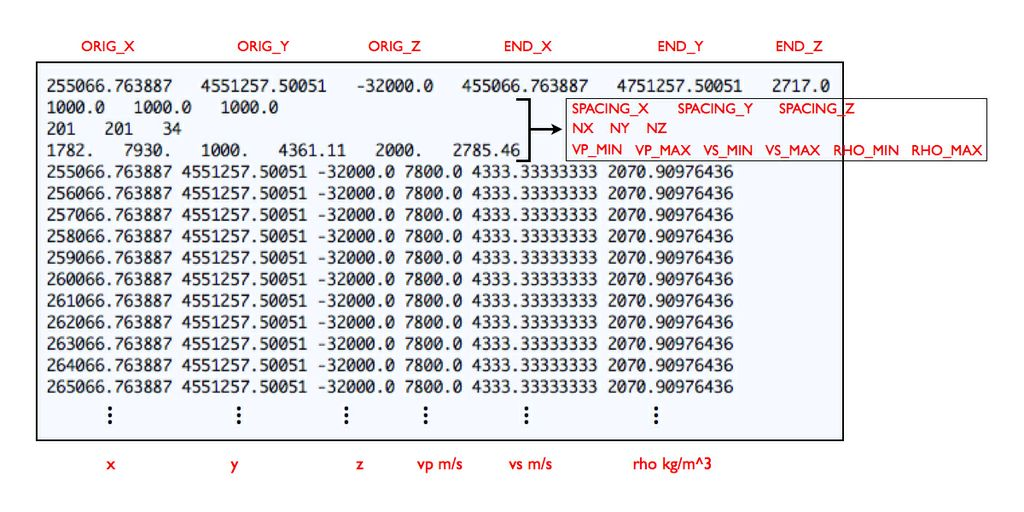
\includegraphics[width=1\textwidth]{figures/tomo_file.jpg}
\par\end{centering}

\caption{Tomography file \texttt{file\_name} that describes an external, purely elastic Earth
model. The coordinates x, y and z of the grid, their limits ORIG\_X,
ORIG\_Y, ORIG\_Z, END\_X, END\_Y, END\_Z and the grid spacings SPACING\_X,
SPACING\_Y, SPACING\_Z should be in the units of the constructed mesh
(e.g., UTM coordinates in meters).}


\label{fig:tomography_file}
\end{figure}


The user can implement his own interpolation algorithm for the tomography
model by changing the routine \texttt{model\_tomography.f90} located
in the \texttt{src/generate\_databases/} directory. Moreover, for
models that involve both fully defined materials and a tomography
description, the \texttt{nummaterial\_velocity\_file} has multiple
lines each with the corresponding suitable format described above.

%==============

\subsubsection*{Example: External tomography file with variable discretization intervals}

The example in Figure~\ref{fig:tomography_file} is for an external tomography file with uniform spacing in the $x$, $y$, and $z$ directions. (Note that $\Delta x$, $\Delta y$, and $\Delta z$ need not be the same as in the example.) In that example, the  \texttt{nummaterial\_velocity\_file} is
%
\begin{verbatim}
2  -1 tomography elastic tomography_model.xyz 1
\end{verbatim}
%
and the file \texttt{tomography\_model.xyz} will need to reside in \texttt{DATA/}. All entries in the second column of \texttt{materials\_file} will be \texttt{-1}, which means that each element in the mesh will be interpolated according to the values in \texttt{tomography\_model.xyz}.

In some cases it may be desirable to have an external tomography model that is described in more than one file. For example, in cases like southern California, the length scale of variation in the structure of the wave speed model is much shorter in the sedimentary basin models within the upper 15~km. Therefore one might want to use an external tomography file that is sampled with, say, $\Delta x = 1000$~m, $\Delta y = 1000$~m, and $\Delta z = 250$~m in the uppermost 15~km, and then use $\Delta x = 2000$~m, $\Delta y = 2000$~m, and $\Delta z = 1000$~m below a depth of 15~km. If these intervals are chosen appropriately, then it will result in a pair of external tomography file that is much smaller than the alternative of having a single file with the fine discretization. In this case  \texttt{nummaterial\_velocity\_file} is
%
\begin{verbatim}
2  -1 tomography elastic file_above_15km.xyz 1
2  -2 tomography elastic file_below_15km.xyz 1
\end{verbatim}
%
and the files \texttt{file\_above\_15km.xyz} and \texttt{file\_below\_15km.xyz} will need to reside in \texttt{DATA/}.  All entries in the second column of \texttt{materials\_file} will need to be either \texttt{-1} or \texttt{-2}, depending on whether the element is above or below 15~km depth. In this sense, the construction of the mesh and the discretization of the external model will generally be done in tandem.

Other more complicated discretizations can be used following the same procedure. (In particular, there is no limit on the number of different external files that are used.)

%=============


\section{External (an)elastic Models}\label{sec:Anelastic-Models}

To use your own external model, you can set in the \texttt{Par\_file}
the model parameter \texttt{MODEL = external}. Three-dimensional acoustic
and/or (an)elastic (attenuation) models may then be superimposed onto
the mesh based upon your subroutine in \texttt{model\_external\_values.f90}
located in directory \texttt{src/generate\_databases}. The call to
this routine would be as follows
\begin{verbatim}
call model_external_values(xmesh, ymesh, zmesh, &
            rho, vp, vs, qkappa_atten, qmu_atten, iflag_aniso, idomain_id)
\end{verbatim}
Input to this routine consists of:
\begin{description}
\item [{\texttt{xmesh,ymesh,zmesh}}] location of mesh point
\end{description}
Output to this routine consists of:
\begin{description}
\item [{\texttt{rho,vp,vs}}] isotropic model parameters for density $\rho$
($kg/m^{3}$), $v_{p}$ ($m/s$) and $v_{s}$ ($m/s$)
\item [{\texttt{qkappa\_atten,qmu\_atten}}] Bulk and shear wave quality factor: $0<Q_{\kappa,\mu}<9000$
\item [{\texttt{iflag\_aniso}}] anisotropic model flag, $0$ indicating
no anisotropy or $1$ using anisotropic model parameters as defined
in routine file \texttt{model\_aniso.f90}
\item [{\texttt{idomain\_id}}] domain identifier, $1$ for acoustic, $2$
for elastic, $3$ for poroelastic materials.
\end{description}
Note that the resolution and maximum value of anelastic models are
truncated. This speeds the construction of the standard linear solids
during the meshing stage. To change the resolution, currently at one
significant figure following the decimal, or the maximum value (9000),
consult \texttt{shared/constants.h}.



\section{Anisotropic Models}\label{sec:Anisotropic-Models}

To use your anisotropic models, you can either set in the \texttt{Par\_file}
the model parameter \texttt{ANISOTROPY} to \texttt{.true.} or set
the model parameter \texttt{MODEL = aniso}. Three-dimensional anisotropic
models may be superimposed on the mesh based upon the subroutine in
file \texttt{model\_aniso.f90} located in directory \texttt{src/generate\_databases}.
The call to this subroutine is of the form
\begin{verbatim}
call model_aniso(iflag_aniso, rho, vp, vs, &
                 c11,c12,c13,c14,c15,c16,c22,c23,c24,c25,c26, &
                 c33,c34,c35,c36,c44,c45,c46,c55,c56,c66)
\end{verbatim}
Input to this routine consists of:
\begin{description}
\item [{\texttt{iflag\_aniso}}] flag indicating the type of the anisotropic
model, i.e. $0$ for no superimposed anisotropy, $1$ or $2$ for
generic pre-defined anisotropic models.
\item [{\texttt{rho,vp,vs}}] reference isotropic model parameters for density
$\rho$, $v_{p}$ and $v_{s}$.
\end{description}
Output from the routine consists of the following non-dimensional
model parameters:
\begin{description}
\item [{\texttt{c11,..,c66}}] 21~dimensionalized
anisotropic elastic parameters.
\end{description}
You can replace the \texttt{model\_aniso.f90} file by your own version
\textit{provided you do not change the call structure of the routine},
i.e., the new routine should take exactly the same input and produce
the required relative output.



\section{Using external SEP models}\label{sec:Using-SEP}

Stanford Exploration Project (SEP) models consists of two files per variables, one header file (\texttt{.H})
and one binary file (\texttt{.H$@$}).
Among other information, the header file indicates, for each dimension,
the offset (\texttt{o1}, \texttt{o2} and \texttt{o3} fields),
the spatial step size (\texttt{d1}, \texttt{d2} and \texttt{d3} fields)
and the number of samples (\texttt{n1}, \texttt{n2} and \texttt{n3}) necessary to read
the linked binary file (\texttt{in} field).

SEP model reading occurs during database generation. It it the user responsibility
to ensure that proper interfaces between acoustic and elastic domains are set up
during the meshing phase. For more information, refer to
section~\ref{cha:Running-the-Mesher-Meshfem3D}.

In \texttt{DATA/Par\_file}, \texttt{\textbf{MODEL}} should be set to \texttt{\textbf{sep}},
and \texttt{\textbf{SEP\_MODEL\_DIRECTORY}} should point to wherever your sep model files reside.

Note that in order not to overload the parameter file, SEP header files
should be named \texttt{vp.H}, \texttt{vs.H} and \texttt{rho.H}. The \texttt{in} field
in these binary files can be any path as long as it is relative to
the previously set \texttt{SEP\_MODEL\_DIRECTORY}.
We also assume that any dimensional value inside SEP header files is given in meters and
that binary files are single precision floating point numbers stored in little endian format.
There is currently only support for \texttt{vp}, \texttt{vs} and \texttt{rho} variables.

An example demonstrating the use SEP models is given in:
\texttt{EXAMPLES/meshfem3D\_examples/sep\_bathymetry}.


